\documentclass[11pt]{report}
% this template is originally from Roy Dong's ECE 515.
% Edited by Dawei Sun
%%%%%%%%%%%%%%%%%%%%%%%%%%%%%%%%%%%%%%%%%%%%%%%%%%%%%%%%%%%%%%%%%%
% Set the margins of our document.
\usepackage[margin = 1 in]{geometry}

%%%%%%%%%%%%%%%%%%%%%%%%%%%%%%%%%%%%%%%%%%%%%%%%%%%%%%%%%%%%%%%%%%
% Import commands for custom header.
\usepackage{fancyhdr}
\pagestyle{fancy}

%%%%%%%%%%%%%%%%%%%%%%%%%%%%%%%%%%%%%%%%%%%%%%%%%%%%%%%%%%%%%%%%%%
% Allow ourselves to do equations!
\usepackage{amsmath,amssymb,amsthm,amsfonts}
\usepackage{upgreek}
\usepackage{mathtools}

%%%%%%%%%%%%%%%%%%%%%%%%%%%%%%%%%%%%%%%%%%%%%%%%%%%%%%%%%%%%%%%%%%
% Nicer formatting for enumerate commands.
\usepackage[shortlabels]{enumitem}

\usepackage{algorithm2e}
\usepackage[noend]{algpseudocode}

%%%%%%%%%%%%%%%%%%%%%%%%%%%%%%%%%%%%%%%%%%%%%%%%%%%%%%%%%%%%%%%%%%
% Colored text and include images.
\usepackage{color}
\usepackage{graphicx}
\usepackage{float}

\usepackage{listings}
\usepackage{multicol}
%%%%%%%%%%%%%%%%%%%%%%%%%%%%%%%%%%%%%%%%%%%%%%%%%%%%%%%%%%%%%%%%%%
% Some custom macros to make life easier.
\newcommand{\mc}{\mathcal}
\newcommand{\mb}{\mathbb}

\newcommand{\T}{\intercal}
\newcommand{\E}[1]{\mathbb{E}\left[#1\right]}

%%%%%%%%%%%%%%%%%%%%%%%%%%%%%%%%%%%%%%%%%%%%%%%%%%%%%%%%%%%%%%%%%%
%%%%%%%%%%%%%%%%%%%%%%%%%%%%%%%%%%%%%%%%%%%%%%%%%%%%%%%%%%%%%%%%%%
%%%%%%%%%%%%%%%%%%%%%%%%%%%%%%%%%%%%%%%%%%%%%%%%%%%%%%%%%%%%%%%%%%

\lhead{CS598SM - Fall 2020 at University of Illinois at Urbana-Champaign}
\rhead{\textcolor{red}{Dawei Sun (daweis2)}}

%%%%%%%%%%%%%%%%%%%%%%%%%%%%%%%%%%%%%%%%%%%%%%%%%%%%%%%%%%%%%%%%%%
%%%%%%%%%%%%%%%%%%%%%%%%%%%%%%%%%%%%%%%%%%%%%%%%%%%%%%%%%%%%%%%%%%
%%%%%%%%%%%%%%%%%%%%%%%%%%%%%%%%%%%%%%%%%%%%%%%%%%%%%%%%%%%%%%%%%%

\begin{document}

%%%%%%%%%%%%%%%%%%%%%%%%%%%%%%%%%%%%%%%%%%%%%%%%%%%%%%%%%%%%%%%%%%
%%%%%%%%%%%%%%%%%%%%%%%%%%%%%%%%%%%%%%%%%%%%%%%%%%%%%%%%%%%%%%%%%%
%%%%%%%%%%%%%%%%%%%%%%%%%%%%%%%%%%%%%%%%%%%%%%%%%%%%%%%%%%%%%%%%%%
\section*{Problem 1}
\paragraph{(1)} The original function and its approximation are shown in the following figure. Approximation is not accurate outside $[-\pi, \pi]$.
\begin{figure}[h!]
    \centering
    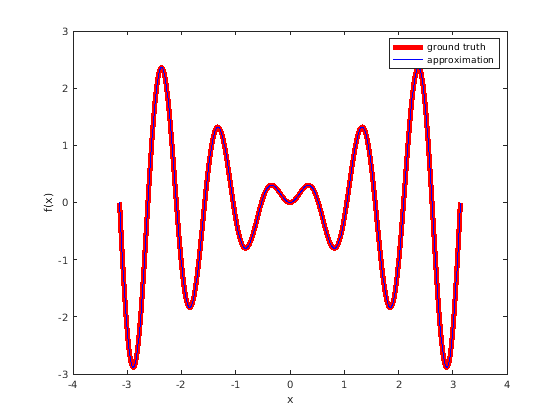
\includegraphics[width=0.49\linewidth]{CS598SMPPL/hw1/1.1.png}
    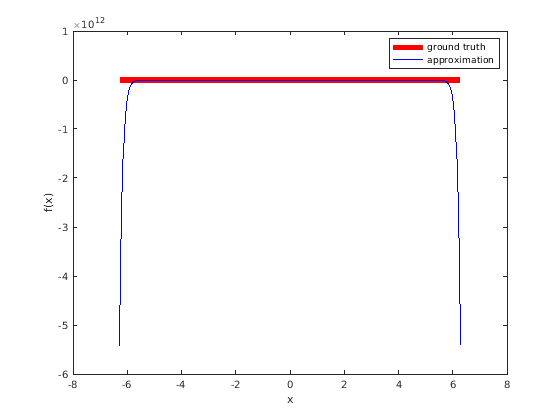
\includegraphics[width=0.49\linewidth]{CS598SMPPL/hw1/1.1_out.png}
    \caption{Left: plot on $[-\pi, \pi]$. Right: plot on $[-2\pi, 2\pi]$.}
\end{figure}

\paragraph{(2)}
As shown in the following figure, approximation error looks periodic. As the number of significant digits $n$ increases, approximation error decreases but is finally saturated.
\begin{figure}[H]
    \centering
    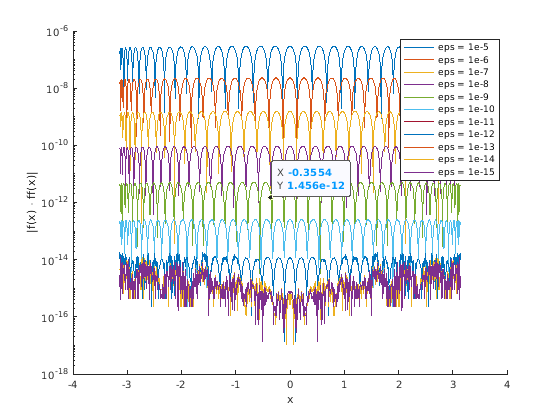
\includegraphics[width=0.8\linewidth]{CS598SMPPL/hw1/1.2.png}
    \caption{Approximation error for different numbers of significant digits $n$. Here, eps = $10^{-n}$.}
\end{figure}

\section*{Problem 2}
Compared to tanh, approximating sigmoid requires fewer Chebyshev terms. This may be because that sigmoid is more smooth, i.e. the maximum of the absolute value of its derivative is smaller.

\noindent The function object used in the experiments is as follows
\begin{verbatim}
sigmoid = @(x) (1 ./ (1 + exp(-x)));
ff = @(x) sigmoid(8*(x-.5)) + 1e-6*sin((1:length(x))'.^2);
\end{verbatim}
Directly approximating it without specifying the argument eps does not work. Thus, we use the eps argument. In the following figures, we compare the results of $eps = 10^{-6}, 10^{-9}, 10^{-3}$ with the result of $eps = 10^{-6}$ and doublelength=True. Again, $eps = 10^{-12}$ does not work.
\begin{figure}[h!]
    \centering
    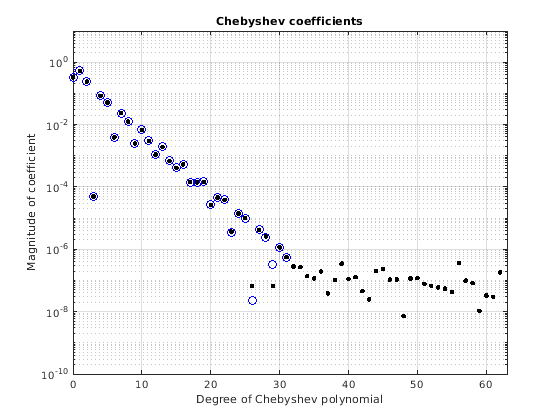
\includegraphics[width=0.32\textwidth]{CS598SMPPL/hw1/2.1.png}
    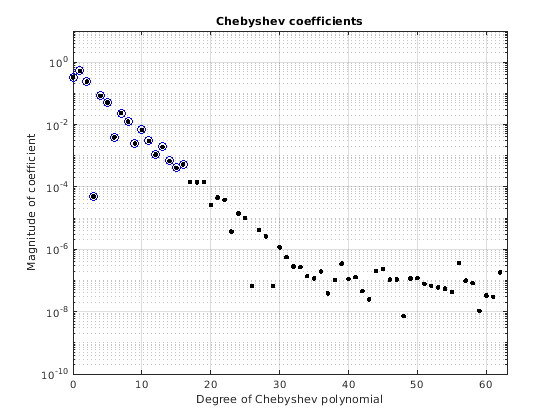
\includegraphics[width=0.32\textwidth]{CS598SMPPL/hw1/2.2.png}
    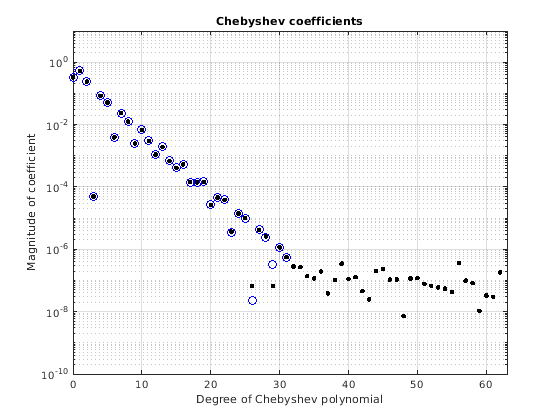
\includegraphics[width=0.32\linewidth]{CS598SMPPL/hw1/2.3.png}
    \caption{Form Left to Right. 1. $eps = 10^{-6}$; 2. $eps = 10^{-3}$; 3. $eps = 10^{-9}$.}
\end{figure}

\noindent Next, we study the following function.
\begin{verbatim}
gg = @(x) sigmoid(8*(x-.5)) + 1e-6*sin(200*exp(x));
\end{verbatim}
We show the results in the following figures.
\begin{figure}[h!]
    \centering
    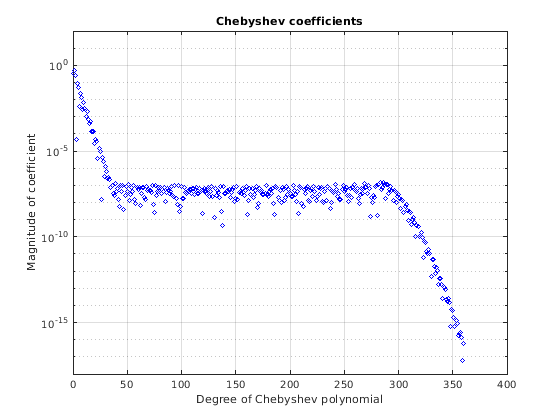
\includegraphics[width=0.45\linewidth]{CS598SMPPL/hw1/2.4.png}
    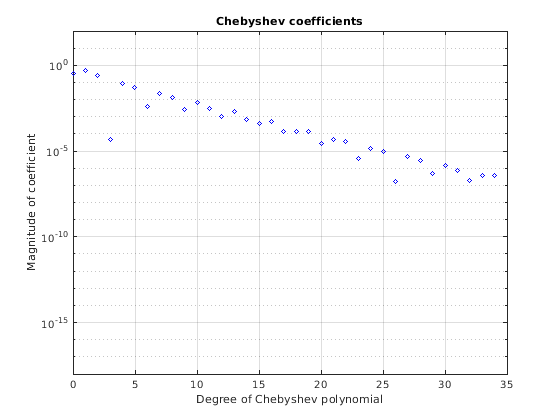
\includegraphics[width=0.45\linewidth]{CS598SMPPL/hw1/2.5.png}
    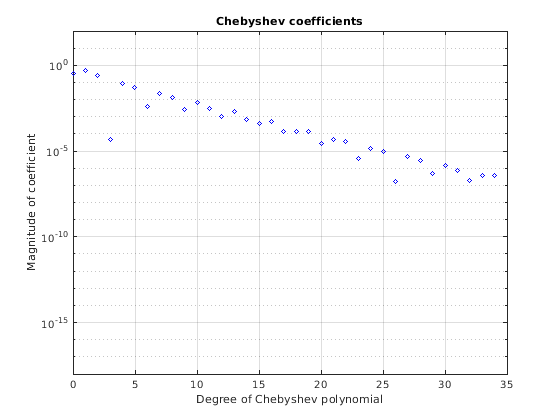
\includegraphics[width=0.45\linewidth]{CS598SMPPL/hw1/2.6.png}
    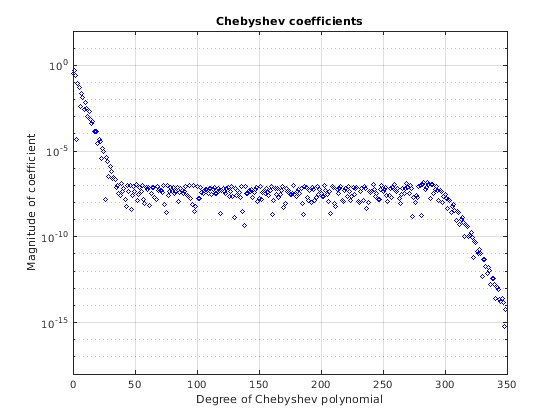
\includegraphics[width=0.45\linewidth]{CS598SMPPL/hw1/2.7.png}
    \caption{Form Left to Right and Top to Bottom. 1. eps is automatically determined by Chebfun; 2. $eps = 10^{-6}$; 3. $eps = 10^{-9}$; 4. $eps = 10^{-12}$.}
\end{figure}

\section*{Problem 3}
If we want to use Chebfun to approximate log function on an interval $[\epsilon, 1]$, we may encounter a problem if $\epsilon$ is too small. In that case, the derivative may be very large and approximating this function may require more than 65537 points. For example, chebfun does not work in the following case.
\begin{verbatim}
eps=1e-8;
chebfun(@(x) log(x), [eps, 1])
\end{verbatim}
\end{document}
